\documentclass{article}

\usepackage{listings}
\usepackage{hyperref}
\usepackage{amsmath}
\usepackage{pgf}
\usepackage{tikz}
\usetikzlibrary{arrows,shapes,snakes,automata,backgrounds,petri,matrix,plotmarks}
\usepackage{xcolor}


%%% datas
\begin{filecontents}{knn.1.igndata}
    1  1
    2  3
    10 13
    20 18
    14 9
\end{filecontents}
\begin{filecontents}{knn.2.igndata}
    10  1
    20  3
    1  13
    2  18
    1  9
\end{filecontents}

\title{The Summary of Machine Learning}
\author{John Lee \\  me@qinka.pro \\ qinka@live.com}

\begin{document}
\maketitle
\begin{abstract}
  This report is mainly about basic algorithms for machine learning,
  including supervised classification, supervised regression, and unsupervised clustering.
  The mainly algorithms are decision tree, k-nearest negihbor, support vector machine, nerual network,
  linear-regression, k-means, hierarchial, and convolution nerual network.
  Most of these algorithms will be instanced with Haskell, and most of them are applied to NAO robot.
  All the codes and this report are opend on GitHub, with GNU's
  \href{https://www.gnu.org/copyleft/gpl.html}{GPLv3+} license and GNU's
  \href{https://www.gnu.org/licenses/quick-guide-gplv3.html}{FDL}.
\end{abstract}
\section*{Copyleft}
\label{sec:copyleft}

All of these codes and documents are under GNU's GPLv3+ and FDLv1.3+. \\
{\large Copyleft (C) 2017 John Lee <me@qinka.pro> <qinka@live.com>} \\

\paragraph{Notice for Codes}

All the codes in the reimagined-pancake are under GPLv3+ license.

Reimagined-Pancake is a serial toy about machine learning and NAO robot.
Copyright (C) 2017 John Lee <me@qinka.pro> <qinka@live.com>

This program is free software: you can redistribute it and/or modify
it under the terms of the GNU General Public License as published by
the Free Software Foundation, either version 3 of the License, or
(at your option) any later version.

This program is distributed in the hope that it will be useful,
but WITHOUT ANY WARRANTY; without even the implied warranty of
MERCHANTABILITY or FITNESS FOR A PARTICULAR PURPOSE.  See the
GNU General Public License for more details.

You should have received a copy of the GNU General Public License
along with this program.  If not, see \href{http://www.gnu.org/licenses}{<http://www.gnu.org/licenses/>}.

\paragraph{Notice for Documents and Reports}

In reimagined-pancake, all the documents(not including the one in the codes), reports and other texts,
are under the GNU's FDLv1.3+ license.

This report is a summary, or say a report about the machine.

Copyright (C)  2017 John Lee <me@qinka.pro> <qinka@live.com>

Permission is granted to copy, distribute and/or modify this document
under the terms of the GNU Free Documentation License, Version 1.3
or any later version published by the Free Software Foundation;
with no Invariant Sections, no Front-Cover Texts, and no Back-Cover Texts.
A copy of the license is included in the section entitled "GNU
Free Documentation License".

You should have received a copy of the GNU Free Documentation License
along with this program.  If not, see \href{http://www.gnu.org/licenses}{<http://www.gnu.org/licenses/>}.

\section{Decision Tree}
\label{sec:decisiontree}

For the first algorithm about machine learning, let's talk about decision tree.

The decision tree is just like a state machine or flow chart, and it is a like of decision support tool
by using a tree-like graph or model to help people make decision, while it can also help machine.

The way it works is that in the each node, there is a if-condition, and when it's true it will move to
one of sub-node. When it's false, it will move to another sub-node. When it moves to the end-node,
that means there is a decision which we can make.

For example, if you want to know whether you need to take an umbrella, the ``if-condition'' is
whether it's raining outside. If the condition is true, you need to move to end-node, ``take an umbrella'',
and if not, you need to move to the end-node, ``leave umbrella alone''.
If it's drawn as a graph, it will likely be figure\ref{fig:dt:eg}.

\begin{figure}
  \centering
  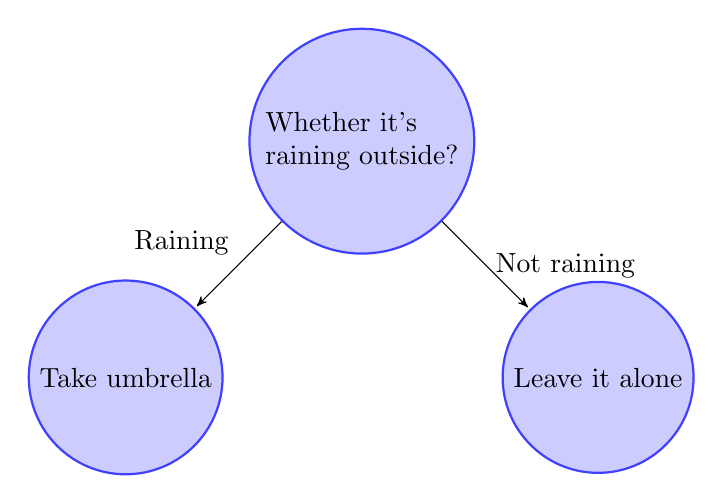
\begin{tikzpicture}[node distance=3cm,>=stealth',bend angle=20,auto]        
    \tikzstyle{point}=[circle,thick,draw=blue!75,fill=blue!20,minimum size=6mm]
    \begin{scope}
      \node[point](rain){\vbox{\hbox{Whether it's}\hbox{raining outside?}}};
      \node[point,below of=rain,left of=rain](take){Take umbrella}
      edge [pre] node {Raining} (rain);
      \node[point,below of=rain,right of=rain](leave){Leave it alone}
      edge [pre,right] node {Not raining} (rain);
    \end{scope}
  \end{tikzpicture}
  \caption{The decision tree for example.}
  \label{fig:dt:eg}
\end{figure}

\subsection{How Does Machine Learning?}
\label{sec:dt:how}

First of all, we need to know what entropy is.
Then we will talk about ID3 algorithm to learning a decision tree.

\subsubsection{Entropy}
\label{sec:dt:how:entropy}

Entropy was defined to represent the ``size'', or say amount of informations.
Simply, it represent how many bit are needed to encode a serial of informations.
The equation of the entropy is equation.\ref{eq:entroy}.
\begin{equation}
  \label{eq:entropy}
  H(X) = - \sum\limits_x P(x)\log_2\left[P(x)\right]
\end{equation}
And that means the entropy will be larger when the variable's more uncertain.
The unit of entropy is bit.

For example, there is an asymmetrical coin. The probability of frontage is 0.8,
while that of other size is 0.2.
So the entropy is $H(X) = - 0.2\log_20.2 - 0.8\log_20.8 = 0.7219$.

\subsubsection{ID3}
\label{sec:dt:how:id3}

When there are many attributes which can be used as ``if-condition'',
we need to find out one of them as the node. So the information gain is defined.
\begin{equation}
  \label{eq:inforgain}
  Gain(A) = Info(D) - Info_A(D)
\end{equation}
where $A$ means one of the attributes, and $Info$ means simply entropy.
The $Info_A$ means the average entropy for each range of age.
The difference means how many informations we can ``get'' if ``split'' by age.

So the basic idea of ID3 algorithm is 
\begin{quote}
  For each node, find out which attribute's \textit{information gain} is the largest.
  If there is not any attribute or all item in this node belongs to one class, this node is a end-node.
  If there is a attribute's information gain is the largest, the tree will be split by this attribute.
  And then do it again until we get all the end-node.
\end{quote}

\section{K-Nearest Neighbor}
\label{sec:knn}

K-Nearest Neighbor uses distence to classify. For an item, the k-nearest neighbors will be use
to classify.
\begin{figure}
  \centering
  \begin{tikzpicture}[only marks, y=.3cm,x=.3cm]
  %axis
  \draw (0,0) -- coordinate (x axis mid) (22,0);
  \draw (0,0) -- coordinate (y axis mid) (0,22);
  \draw plot[mark=*,mark options={fill=white}] file {knn.1.igndata};
  \draw plot[mark=*] file {knn.2.igndata};
  \draw plot[mark=square*, mark options={fill=white}] (10,10);
  \draw [dashed] (10,10) circle [radius=5];
  \end{tikzpicture}
  \caption{Example of k-NN classifcation, where k = 2}
  \label{fig:knn:eg}
\end{figure}
For example, in the figure \ref{fig:knn:eg}, when the $k=2$, the item should be same with white one.

\subsection{How to learning?}
\label{sec:knn:learning}

The first step is computing the distances between item, which need to be classified, and training datas.
The second step is finding out which class the most of k-nearest neighbors belong to.

Normally, we can use \textbf{euclidean distance}, \textbf{cosine}, \textbf{correlation},
or \textbf{manhattan distance} to measure the distance.

\section{Support Vector Machine}
\label{sec:svm}

Support vector machines are supervised learning models. It's mainly used to classify,
while it can also be use to regression analysis.
The basic ideas of support vector machine are
\begin{itemize}
\item Mapping data to higher-dimensional linear-separable feature space
\item Finding out the best hyperplane to split data
\end{itemize}

\subsection{Kernel Function}
\label{sec:svm:kf}

To map the samples to the feature space, there are many ways to do it.
However, it is possible that samples are mapped to a infiniet-dimensional space.
For example, we can use $\phi(x)=(1,x,x^2,x^3,\dots)^T$ to map samples to a infiniet-dimensional space.
But that is bad idea, because it is impossible to compute.
So we need to use kernel function to map.

So let me tell you how to use kernel function.
The kernel function is dualistic function $K(\cdot,\cdot)$.
For samples $\{(\mathbf{x}_i,y_i)\}^n_{i=1}$, and kernel function(s) $K(\mathbf{x},\mathbf{x}_j)^n_{j=1}$,
the mapping function will be defined as
\begin{equation}
  \label{eq:mapping}
  f_\theta(\mathbf{x})=\sum\limits_{j=1}^{n}\theta K(\mathbf{x},\mathbf{x}_k)
\end{equation}
There are some popular kernel function:
\begin{itemize}
\item linear
  \begin{equation}
    \label{eq:kf:linear}
    K(\mathbf{x}_i,\mathbf{x}_j) = \mathbf{x}_i^T\mathbf{x}_j
  \end{equation}
\item polynomial
  \begin{equation}
    \label{eq:kf:polynomial}
    K(\mathbf{x}_i,\mathbf{x}_j) = \left(\gamma \mathbf{x}_i^T\mathbf{x}_j+r\right)^d,\gamma > 0
  \end{equation}
  %% 径向基函数
\item radial basis function
  \begin{equation}
    \label{eq:kf:rbf}
    K(\mathbf{x}_i,\mathbf{x}_j) = \exp{\left(-\gamma||\mathbf{x}_i-\mathbf{x}_j||^2\right)},\gamma > 0
  \end{equation}
\item sigmoid
  \begin{equation}
    \label{eq:kf:sigmoid}
    K(\mathbf{x}_i,\mathbf{x}_j) = \tanh{\left(\gamma \mathbf{x}_i^T\mathbf{x}_j+r\right)}
  \end{equation}
\end{itemize}
where $\gamma$,$r$, and $d$ are kernel parameters.

\subsection{Hyperplane}
\label{sec:svm:hyperplane}

The hyperplane used to classify should have the largest distances to it's nearest training-data.

So, one of model to represent hyperplane is:
$$
\mathbf{x} = \left[\begin{array}{c} x_1 \\ x_2 \\ \vdots \\ x_d \end{array}\right];
\mathbf{w} = \left[\begin{array}{c} w_1 \\ w_2 \\ \vdots \\ w_d \end{array}\right];
h(\mathbf{x}) = sign\left(\mathbf{w}^T\mathbf{x}+b\right)
$$
It is, at the same times, also a optimization problem, and the model is:
\begin{equation}
\label{eq:hyp:op}
\begin{array}{rl}
  \min\limits_{\mathbf{w},b,\mathbf{\xi}} & \frac{1}{2}\mathbf{w}^T\mathbf{w}+C\sum\limits_{i=1}^{l}\xi_i\\
  \text{subject to} & y_i\left(\mathbf{w}^T\phi(\mathbf{x}_i)+b\right) \geq 1 - \xi_i,\\
                                          & \xi_i \geq 0.
\end{array}
\end{equation}

\subsection{How to learn?}
\label{sec:svm:how}

The best way to find out that hyperplane is find the solution of that optimization problem.
By using Lagrange multiplier method:
\begin{equation}
  \label{eq:lagrange-multiplier-method}
  L(\omega,\gamma,\xi,\alpha,\beta) =
  \frac{1}{2}
\end{equation}



\end{document}